%----------------------------------------------------------------------------------------
%	PACKAGES AND OTHER DOCUMENT CONFIGURATIONS
%----------------------------------------------------------------------------------------

\documentclass[paper=a4, fontsize=11pt]{scrartcl} % A4 paper and 11pt font size

% ---- Entrada y salida de texto -----

\usepackage[T1]{fontenc} % Use 8-bit encoding that has 256 glyphs
\usepackage[utf8]{inputenc}
%\usepackage{fourier} % Use the Adobe Utopia font for the document - comment this line to return to the LaTeX default

% ---- Idioma --------

\usepackage[spanish, es-tabla]{babel} % Selecciona el español para palabras introducidas automáticamente, p.ej. "septiembre" en la fecha y especifica que se use la palabra Tabla en vez de Cuadro

% ---- Otros paquetes ----
\usepackage{csquotes} %Para permitir el uso de comillas Quotes https://tex.stackexchange.com/questions/36812/isnt-there-any-other-way-of-doing-double-quotes-in-latex-besides
\usepackage[hyphens]{url} % ,href} %para incluir URLs e hipervínculos dentro del texto (aunque hay que instalar href)
\usepackage{hyperref}
\usepackage{color}
\usepackage{graphics,graphicx, floatrow} %para incluir imágenes y notas en las imágenes
\usepackage{graphics,graphicx, float} %para incluir imágenes y colocarlas

\graphicspath {{./img/}}

\usepackage{listings}  %para introducir comandos

\lstdefinestyle{mybash}
{basicstyle=\ttfamily,
  showstringspaces=false,
  commentstyle=\color{red},
  keywordstyle=\color{blue},
  language=bash,
  alsoletter=/,
  basicstyle=\footnotesize,
  numbers=left,
  stepnumber=1,
  showstringspaces=false,
  tabsize=1,
  breaklines=true,
  breakatwhitespace=false,
}
\lstdefinestyle{mysql}
{basicstyle=\ttfamily,
  showstringspaces=false,
  commentstyle=\color{red},
  keywordstyle=\color{blue},
  language=sql,
  basicstyle=\footnotesize,
  numbers=left,
  stepnumber=1,
  showstringspaces=false,
  tabsize=1,
  breaklines=true,
  breakatwhitespace=false,
}


% Para hacer tablas comlejas
%\usepackage{multirow}
%\usepackage{threeparttable}

%\usepackage{sectsty} % Allows customizing section commands
%\allsectionsfont{\centering \normalfont\scshape} % Make all sections centered, the default font and small caps

\usepackage{fancyhdr} % Custom headers and footers
\pagestyle{fancyplain} % Makes all pages in the document conform to the custom headers and footers
\fancyhead{} % No page header - if you want one, create it in the same way as the footers below
\fancyfoot[L]{} % Empty left footer
\fancyfoot[C]{} % Empty center footer
\fancyfoot[R]{\thepage} % Page numbering for right footer
\renewcommand{\headrulewidth}{0pt} % Remove header underlines
\renewcommand{\footrulewidth}{0pt} % Remove footer underlines
\setlength{\headheight}{13.6pt} % Customize the height of the header

\setlength\parindent{0pt} % Removes all indentation from paragraphs - comment this line for an assignment with lots of text

\newcommand{\horrule}[1]{\rule{\linewidth}{#1}} % Create horizontal rule command with 1 argument of height


%----------------------------------------------------------------------------------------
%	TÍTULO Y DATOS DEL ALUMNO
%----------------------------------------------------------------------------------------
\graphicspath{ {img/} }

\title{
\normalfont \normalsize

\includegraphics[width=6cm,height=6cm]{logo}\\
\textsc{\textbf{Bootcamp Especialidad GNU/Linux (2023)}} \\ [25pt] % Your university, school and/or department name(s)
\horrule{0.5pt} \\[0.4cm] % Thin top horizontal rule
\huge Lab 09 - Servidor de Correo \\ % The assignment title
\horrule{2pt} \\[0.5cm] % Thick bottom horizontal rule
}


%https://es.overleaf.com/learn/latex/Inserting_Images
%Ruta relativa de   imagenes

\author{Pedro Antonio Mayorgas Parejo} % Nombre y apellidos

\date{\normalsize\today} % Incluye la fecha actual

%----------------------------------------------------------------------------------------
% DOCUMENTO
%----------------------------------------------------------------------------------------

\begin{document}

\maketitle % Muestra el Título

\newpage %inserta un salto de página

\tableofcontents % para generar el índice de contenidos

\newpage

%----------------------------------------------------------------------------------------
%	Cuestión 1
%----------------------------------------------------------------------------------------

\section{Preparación de DNS}

En primer lugar, tenemos que preparar el servicio DNS, para poder utilizar el registro MX utilizado para los servicios de correo asociados. Así como podemos indicar la preferencia de los servidores de correo, porque podemos indicar más de uno. El valor más bajo de preferencia, es el que mayor prioridad queremos que tenga, por convención se usa el 10, 20, 30...

\begin{figure}[H]
	\centering
	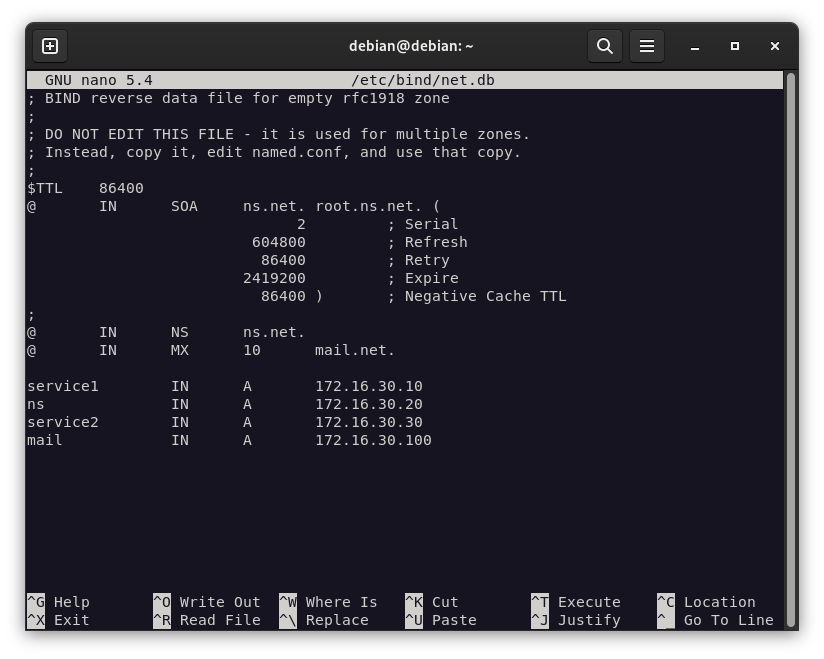
\includegraphics[scale=0.30]{00}
	\caption{Registros de DNS, de la zona.}
\end{figure}


Una vez que hayamos terminado de preparar los registros de la zona MX, también tenemos que indicar el registro A, para que la resolución de DNS, tenga una dirección IP a la que acudir. La siguiente captura son las pruebas, donde usamos el comando dig, para obtener un servidor de correo con el registro MX de la zona.

\begin{figure}[H]
	\centering
	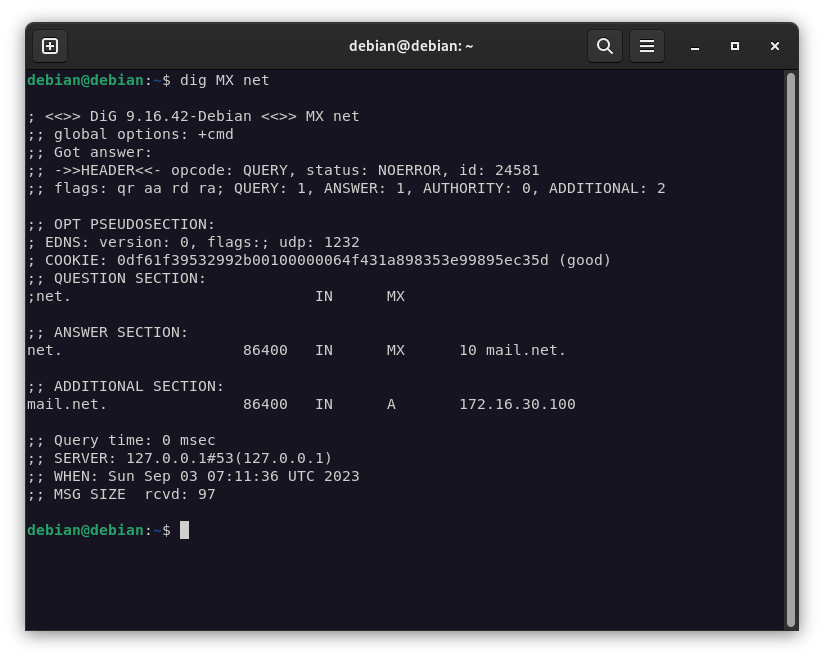
\includegraphics[scale=0.30]{01}
	\caption{Pruebas del servicio DNS.}
\end{figure}


Todos los comandos que han sido utilizados son:

\begin{lstlisting}[style=mybash]
sudo systemctl restart bind9.service
sudo systemctl status bind9.service
\end{lstlisting}

Una vez que se han reiniciado los servicios, debemos también comprobar que se hayan cargado las zonas de DNS correctamente, para ello con el último comando que se ha indicado anteriormente, se debe comproabr que aparezca un \textbf{all zones loaded}.

\section{Instalación de Postfix MTA}

Postfix es un MTA Mail Transfer Agent, que te permite el envío de correos electrónicos por el protocolo SMTP (Simple Mail Transfer Protocol). Es un MTA muy robusto que permite una amplia configuración.
\vspace{5mm}

Para la instalación de Postfix, hemos utilizado una distribución basada en Red Hat, para poder seguir un manual profesional de configuración del MTA. La mayoría de los cambios se han concrentrado en el fichero \textbf{main.cf}, dicho fichero se localiza en \textbf{/etc/postfix/main.cf}. En la documentación de Red Hat se indica que hay que concentrarse en la configuración inicial de los siguientes parámetros del fichero de configuración, para que pueda configurarse de manera básica el MTA.
\vspace{5mm}

Comando para instalar Postfix en las distribuciones Red Hat:

\begin{lstlisting}[style=mybash]
sudo dnf update
sudo dnf install postfix
\end{lstlisting}

\begin{figure}[H]
	\centering
	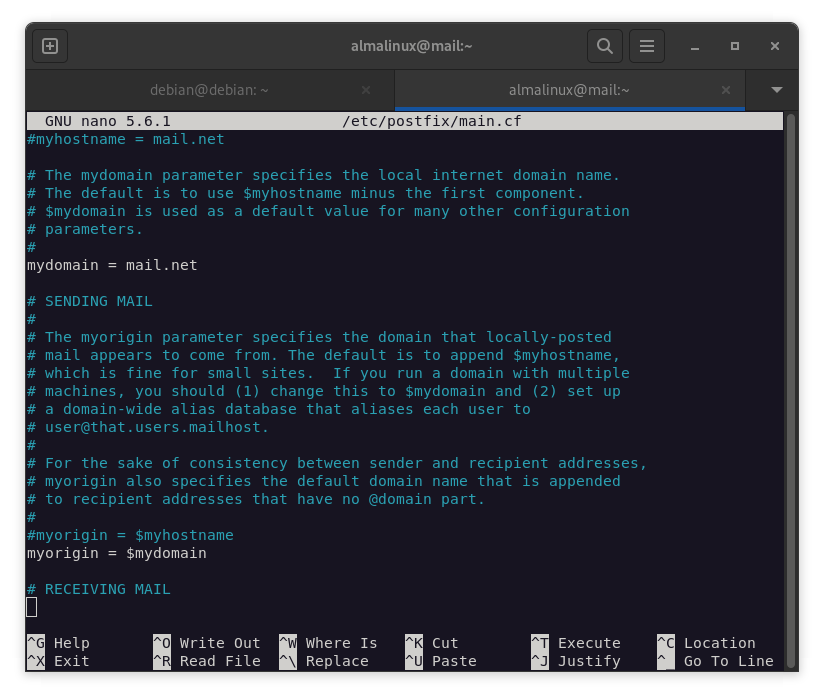
\includegraphics[scale=0.30]{02}
	\caption{Parámetros de main.cf - Configuración del dominio y origen.}
\end{figure}

En la captura anterior, se tiene que configurar el dominio local del servicio de correo. Puede ser mx.dominio.tld, o dominio.tld indistintamente. Luego el siguiente parámetro que hemos configurado, es el de origin, que es el parámetro utilizado para indicar el origen de mensajes enviados desde este MTA o sus usuarios.

\begin{figure}[H]
	\centering
	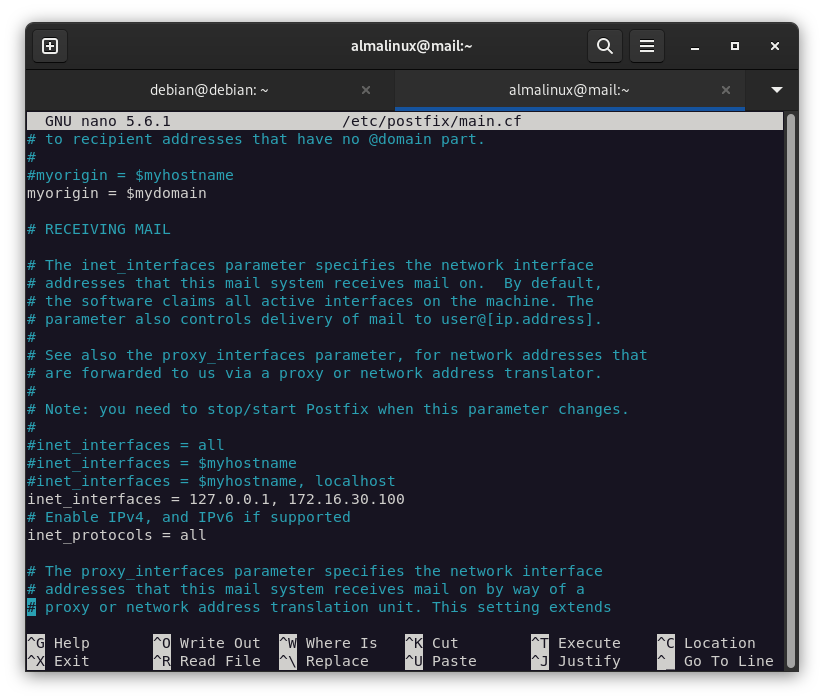
\includegraphics[scale=0.30]{03}
	\caption{Parámetros de main.cf - Configuración de las interfaces de recepción de email.}
\end{figure}

Ahora tenemos que configurar las interfaces por las que Postfix recibe los correos, en el manual de administración se puede indicar un parámetro especial \textbf{all}, pero esto implica que se ponga el correo en escucha en todas las interfaces de red indistintamente,lo cual no suele ser bueno. En su lugar, he configurado dos interfaces, en la cual una es la dirección IP externa y otra que debería de estár de manera obligatoria que es la dirección de loopback o localhost.

\begin{figure}[H]
	\centering
	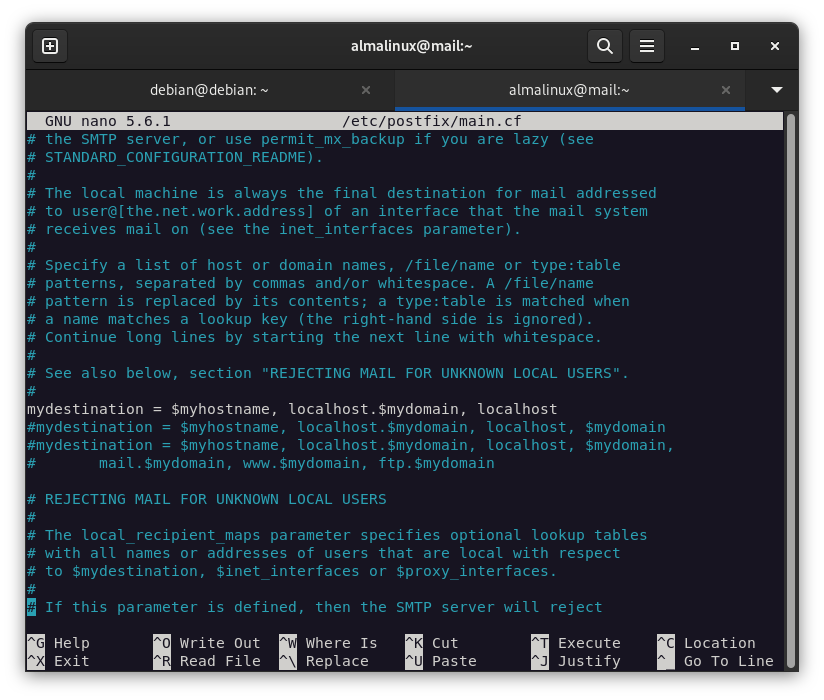
\includegraphics[scale=0.30]{04}
	\caption{Parámetros de main.cf - Configuración de destinatarios en el MTA.}
\end{figure}

Luego tenemos que configurar el parámetro de \textbf{mydestination}, que consiste en cómo acepta de manera interna el MTA que es un destinatario que se envía de manera local, en vez de hacer reenvío. La configuración indicada en el manual de postfix es el caso 1, donde es el caso por defecto.
\vspace{5mm}

Una vez terminada la configuración anterior, debemos ejecutar el comando siguiente para comprobar si la configuración del main.cf de Postfix contiene algún error.

\begin{lstlisting}[style=mybash]
sudo postfix check
\end{lstlisting}

Luego de configurar Postfix, debemos activar y habilitar el servicio con el siguiente comando:

\begin{lstlisting}[style=mybash]
sudo systemctl enable --now postfix.service
# Verify
sudo systemctl status postfix
\end{lstlisting}

Luego tenemos que probar el servicio de correo, para ello instalar la siguiente utilidad que nos permite usar el MTA para enviar correos a los usuarios locales, claro que tenemos que crear previamente al usuario para poder enviarle el mail, así como para poder autenticarnos y leer su correo final en /var/log/maillog o en 
\begin{lstlisting}[style=mybash]
sudo dnf install sendmail
nano mail.txt
sendmail pedro@mail.net < mail.txt
\end{lstlisting}

\begin{figure}[H]
	\centering
	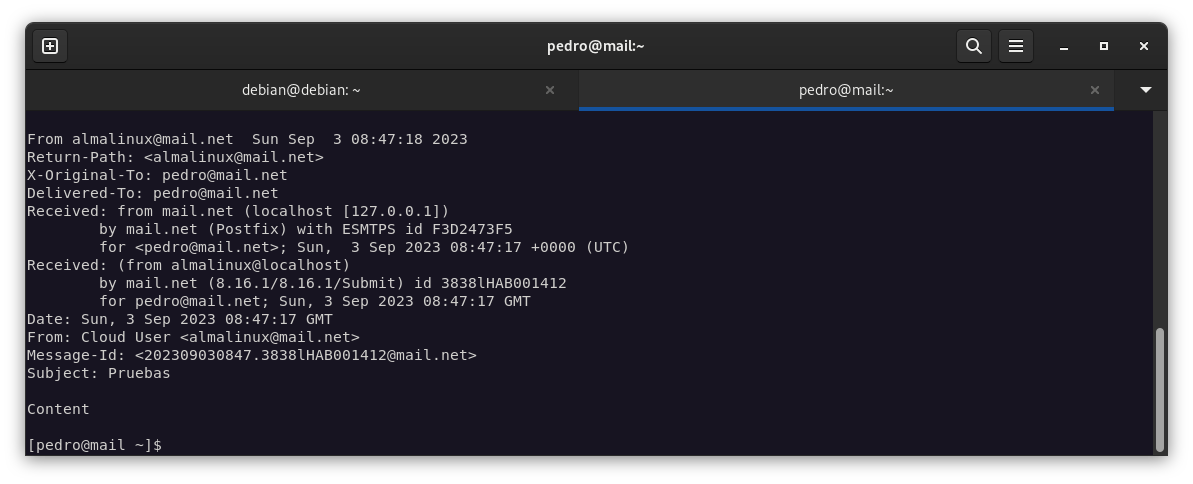
\includegraphics[scale=0.30]{05}
	\caption{Recepción del correo electrónico.}
\end{figure}

Para poder ver los correos, vamos a \textbf{/var/log/mail/\$USER}

\newpage 
\section{Instalación y configuración de Dovecot}

Ahora tenemos que realizar la instalación de Dovecot con el siguiente comando.


%\begin{figure}[H]
%	\centering
%	\includegraphics[scale=0.30]{cuestion_1_1}
%	\caption{Se puede ver que al no haber un fallo grave, el sistema lo nota como que sigue funcionando pero en un estado degradado.}
%\end{figure}

%\newpage

%Se pueden hacer include en latex
%\newpage

\section{Section}

\subsection{Subseccion}

\subsubsection{Subseccion}



%-------Bibliografia-----------------------------

%\newpage
\section{Bibliografía}

% Ejemplo
\footnote{Administración de mdadm - Por Red Hat}
\textcolor{blue}{\url{https://access.redhat.com/documentation/en-us/red_hat_enterprise_linux/8/html/managing_storage_devices/managing-raid_managing-storage-devices#monitoring-raid_managing-raid}}



\end{document}
